\documentclass[dvipdfmx]{jsarticle}
\usepackage{amsmath,amsfonts}
\usepackage{titlesec}
\usepackage{graphicx}
\usepackage{float}
\usepackage{comment}
\usepackage{fancyhdr}
\usepackage{url}

\lhead{}%ヘッダ左上を空白化
\graphicspath{{../fig/}}%\includegraphicsのファイル名省略用
%高さの設定
\setlength{\textheight}{\paperheight}%ひとまず紙面を本文領域に
\setlength{\topmargin}{-5.4truemm}%上の余白を20mm(=1inch-5.4mm)に
\addtolength{\topmargin}{-\headheight}%
\addtolength{\topmargin}{-\headsep}%ヘッダの分だけ本文領域を移動させる
\addtolength{\textheight}{-40truemm}%下の余白も20mmに
%%幅の設定
\setlength{\textwidth}{\paperwidth}%ひとまず紙面を本文領域に
\setlength{\oddsidemargin}{-0.4truemm}%左の余白を20mm(=1inch-5.4mm)に
\setlength{\evensidemargin}{-0.4truemm}%
\addtolength{\textwidth}{-50truemm}%右の余白も20mmに

%図,表の表示名
\renewcommand{\figurename}{Fig. }
\renewcommand{\tablename}{Table }

%図,表,式などの間隔
\setlength{\abovecaptionskip}{1mm}	%図・表とキャプションの間隔の変更
\setlength{\belowcaptionskip}{1mm}
\setlength{\abovedisplayskip}{3pt}%式の上部のマージン
\setlength{\belowdisplayskip}{3pt}%式の下部のマージン

%図番号を(subsection).(図番号)に変更
\makeatletter
\renewcommand{\thefigure}{\thesection.\arabic{figure}}
\@addtoreset{figure}{section}

%表番号を(subsection).(表番号)に変更
\renewcommand{\thetable}{\thesection.\arabic{table}}
\@addtoreset{table}{section}

%式番号を(subsection).(式番号)に変更
\renewcommand{\theequation}{\thesection.\arabic{equation}}
\@addtoreset{equation}{section}
\makeatother

%注釈
\renewcommand\thefootnote{*\arabic{footnote}}

%目次の表示レベル設定
\setcounter{tocdepth}{3}


\renewcommand{\postpartname}{章} %部を章に変更
%\renewcommand{\thepart}{\Roman{part}}  

\begin{document}

\twocolumn[
  \begin{center}
    \vspace{20mm}
    {\huge 研究計画書}\\
    \vspace{5mm}  
    {\Large 車輪に依存しない段差登攀ロボットの開発}\\
    \vspace{5mm}
    {\Large 千葉工業大学 先進工学部 未来ロボティクス学科 米田研究室}\\
    {\Large 学生番号 21C1016 稲葉健}\\
    \vspace{5mm}
    {\Large \today}\\
  \end{center}
]

\section{研究背景}
近年普及の進む掃除ロボットを始めとする室内移動系のロボットは,車輪径・車高を大きくすることが難しいケースも少なくない.
しかし,一般的な車輪ロボットでは,車輪半径の半分以上,車高以上の段差を登攀することは困難である.
そのため,現行の室内移動ロボットの運用は,大きな段差のないフロアを移動することが主である.
% 画像
\begin{figure}[H]
  \centering
  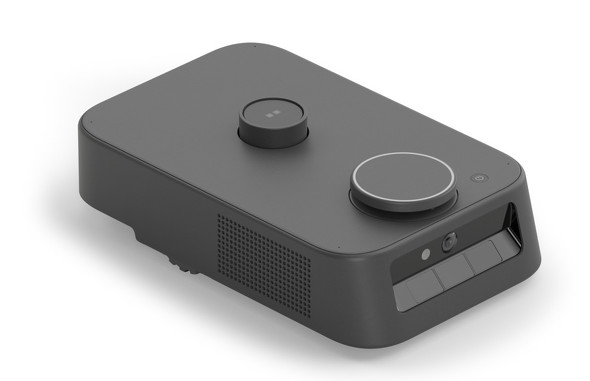
\includegraphics[width=50mm]{image/mn0201_kachaka_006}
  \caption{家庭内を移動するロボット(kachaka)[1]}
  
  \label{fig:runba}
\end{figure}
したがって,室内移動型のロボットを複数階建ての一軒家などで運用する場合,
複数のフロアで稼働させるためには人間がロボットを移動させるか,
複数台のロボットを稼働させる必要がある.
移動させる作業はロボットの重量が増えていくごとに困難になり,
作業中の事故なども懸念される.
また,複数台稼働させるとなると,1台のロボットを導入したメリットを享受できるのが1フロアだけになってしまう.

そこで,車輪で移動を行い,段差の上り下りを車輪に依存せずに行うロボットを開発すれば,
車輪径や車高は別の問題に最適化しつつ,フロア間の移動が可能になるのではないかと考えた.
\section{研究目的}
現在普及の進む掃除ロボットの中には段差登攀性能を売りにしている製品も存在する.
しかし,Fig.\ref{fig:rulo}に示すようにその多くが$20\mathrm{mm}$程度のカーペットやラグなどで生じる小さな段差を想定しており,
階段サイズの段差を登攀可能な製品は少ない.
% 画像
\begin{figure}[H]
  \centering
  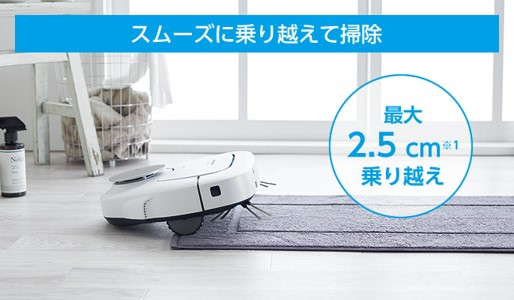
\includegraphics[width=50mm]{image/rulo.jpg}
  \caption{Panasonic RULO[2]}
\label{fig:rulo}
\end{figure}

一般的な階段の段差は約$200\mathrm{mm}$程度であり,奥行きは$300\mathrm{mm}$程度ある.

本研究では一般家庭の階段を連続登攀することを想定し,直径$300\mathrm{mm}$の円内に全長が収まり,
$200\mathrm{mm}$の段差登攀性能を有すロボットの開発を目的とする.
また,車輪径については,iRobot社のルンバの車輪径よりも小さい$55\mathrm{mm}$径のものを使用し,
既存のロボットにも応用可能であることを示す.

\section{研究方法}
段差踏破方法について,二つの台車を用いて互いを持ち上げ合う方式を取る.

Fig.\ref{fig:model01}に示すように,二つの台車をアームで接続し,上の段に登った
台車に重りを移動させ,段差の下の台車を持ち上げることで段差の登攀を完了する.
登攀の際に移動させる重りの条件式である.
% 数式
\begin{equation}
  M=\frac{l'+lcos\theta-l''}{l''}m
\label{equ:model01}
\end{equation}
\begin{table}[H]
    \begin{tabular}{lcl}
      $M$ & : & 移動させる重りの質量[kg]\\
      $m$ & : & 台車の質量[kg]\\
      $l$ & : & 台車間距離[mm]\\
      $l_1$,$l_2$  & : & 台車の支点から重心の距離[mm]\\
      $\theta$ & : & 台車とアームの角度[deg]\\
  \end{tabular}
\end{table}
式(\ref*{equ:model01})より,Mを最小限に抑えるには
持ち上げる瞬間の$lcos\theta$を小さくする必要があることが分かる.
そのため,アームの中央に自由度を追加し,段差の下にある台車を持ち上げる際にはFig.\ref{fig:model02}
の様にアームを畳み込み,モーメントを減少させる.
% 画像
\begin{figure}[H]
  \centering
  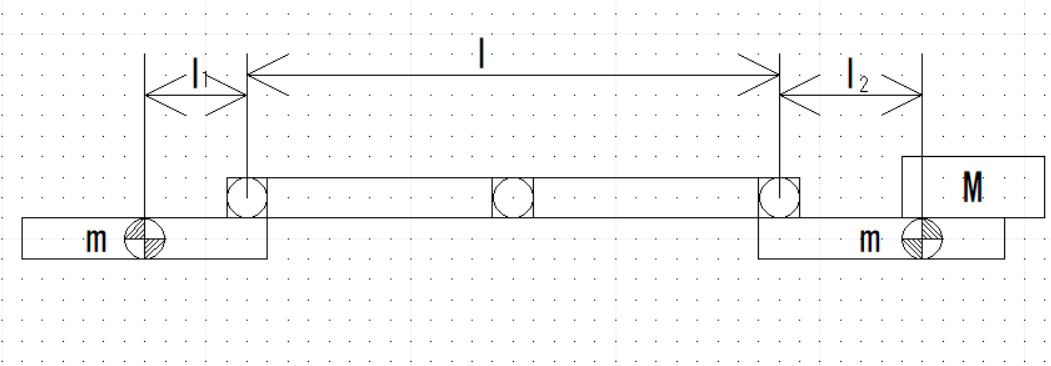
\includegraphics[width=50mm]{image/model01}
  \caption{機体模式図}
\label{fig:model01}
\end{figure}

重りの移動について,アームが3自由度であり,
各台車間の距離が可変になるため,液体をポンプで輸送する方法を採用する.
水を始めとする液体を,
二つの台車についたタンク内を行き来させることで
持ち上げ動作時に接地する台車を切り替え,
段差を登攀する.
% 画像
\begin{figure}[H]
\centering
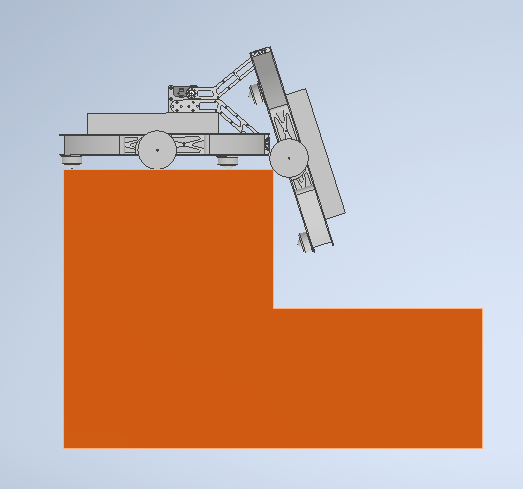
\includegraphics[width=50mm]{image/small_moment}
\caption{段差登攀時の動作イメージ}
\label{fig:model02}
\end{figure}
製作する台車をFig.\ref*{fig:CAD}に示す.
% 画像
\begin{figure}[H]
\centering
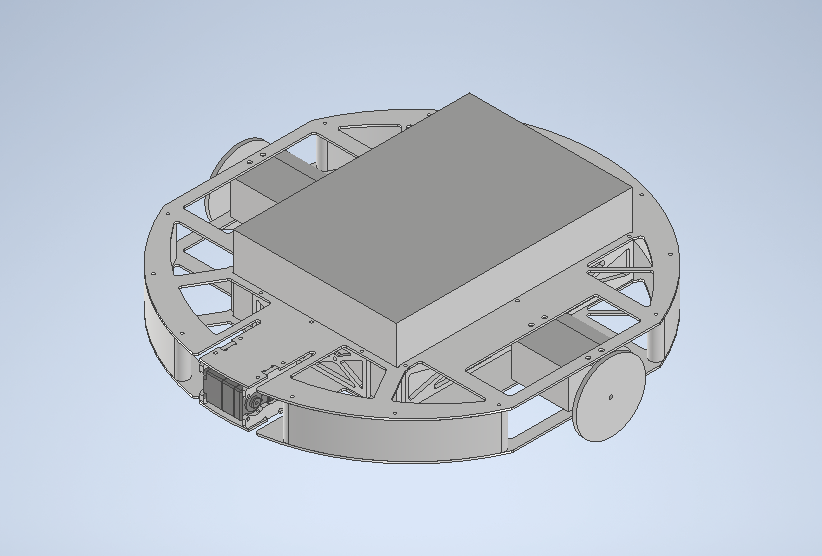
\includegraphics[width=50mm]{image/1unit.png}
\caption{設計した台車}
\label{fig:CAD}
\end{figure}
また,狭い段差内で移動する際の形状をFig.\ref*{fig:move}に示す.

% 画像
\begin{figure}[H]
\centering
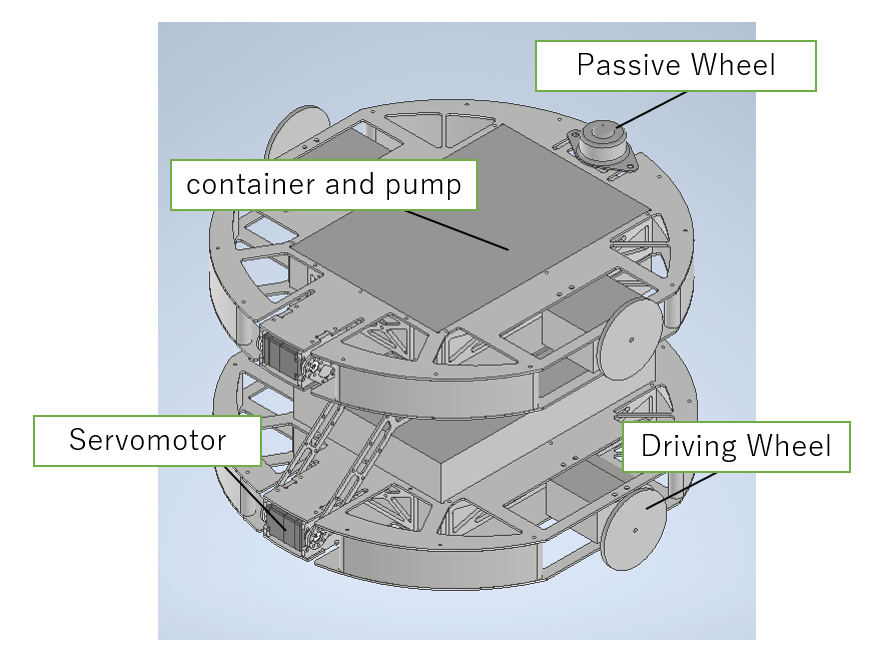
\includegraphics[width=50mm]{image/kasane.png}
\caption{移動時の全体図}
\label{fig:move}
\end{figure}

階段の奥行である$300\mathrm{mm}$以内に収まる様に3自由度のアームを畳み込み,
二つのユニットが重なる形で登攀を開始する.
\section{スケジュール}
今年の6月末までに現在設計中の試作機を完成させ,単純な$200\mathrm{mm}$の段差を登攀する
実験を行う.
現在移動させる質量の参考にしている式から導かれる数値と実際の値を比較し,
式の正誤を確認する.

また,段差を登攀する際にモーメントを最小に抑える軌道を求め,実際の階段での連続登攀実験を行う.

\section{期待される効果}
室内移動型のロボットの行動範囲を広げ,
階段や段差の多い家屋内での運用を押し進める.
また,重心移動機構を個別で取り付けることにより,車輪径以上の溝など
段差以外の障害物を避けることも可能になる可能性がある.
\section{大学院での抱負}
大学院で勉強し,さらに知見を深めることで,
より学術に基づいた設計や制御を行い,
私の製作物のクオリティを挙げていくことができると考える.
また,サークル等で後輩の指導を行った経験を活かし,
研究室内のみならずTAなどの活動で,
よりレベルの高い結果を残せるように後輩たちのサポートを行いたいと考えている.
\section{引用}
\begin{enumerate}
\renewcommand{\labelenumi}{[\arabic{enumi}]}
  \item kachaka\\
        https://store.kachaka.life/products/detail/50\\
        (参照 2024-4-19)
  \item Panasonic ルーロ\\
        https://panasonic.jp/soji/products/rulo.html\\
        (参照 2024-4-18)
  \end{enumerate}
\end{document}
